\documentclass[a4paper]{article}
\usepackage{geometry}
\usepackage{graphicx}
\usepackage{natbib}
\usepackage{amsmath}
\usepackage{amssymb}
\usepackage{amsthm}
\usepackage{paralist}
\usepackage{epstopdf}
\usepackage{tabularx}
\usepackage{longtable}
\usepackage{multirow}
\usepackage{multicol}
\usepackage[hidelinks]{hyperref}
\usepackage{fancyvrb}
\usepackage{algorithm}
\usepackage{algorithmic}
\usepackage{float}
\usepackage{paralist}
\usepackage[svgname]{xcolor}
\usepackage{enumerate}
\usepackage{array}
\usepackage{times}
\usepackage{url}
\usepackage{fancyhdr}
\usepackage{comment}
\usepackage{environ}
\usepackage{times}
\usepackage{textcomp}
\usepackage{caption}
\usepackage{bbm}
\usepackage{enumitem}


\urlstyle{rm}

\setlength\parindent{0pt} % Removes all indentation from paragraphs
\theoremstyle{definition}
\newtheorem{definition}{Definition}[]
\newtheorem{conjecture}{Conjecture}[]
\newtheorem{example}{Example}[]
\newtheorem{theorem}{Theorem}[]
\newtheorem{lemma}{Lemma}
\newtheorem{proposition}{Proposition}
\newtheorem{corollary}{Corollary}

\floatname{algorithm}{Procedure}
\renewcommand{\algorithmicrequire}{\textbf{Input:}}
\renewcommand{\algorithmicensure}{\textbf{Output:}}
\newcommand{\abs}[1]{\lvert#1\rvert}
\newcommand{\norm}[1]{\lVert#1\rVert}
\newcommand{\RR}{\mathbb{R}}
\newcommand{\CC}{\mathbb{C}}
\newcommand{\Nat}{\mathbb{N}}
\newcommand{\br}[1]{\{#1\}}
\DeclareMathOperator*{\argmin}{arg\,min}
\DeclareMathOperator*{\argmax}{arg\,max}
\renewcommand{\qedsymbol}{$\blacksquare$}

\definecolor{dkgreen}{rgb}{0,0.6,0}
\definecolor{gray}{rgb}{0.5,0.5,0.5}
\definecolor{mauve}{rgb}{0.58,0,0.82}

\newcommand{\Var}{\mathrm{Var}}
\newcommand{\Cov}{\mathrm{Cov}}

\newcommand{\vc}[1]{\boldsymbol{#1}}
\newcommand{\xv}{\vc{x}}
\newcommand{\Sigmav}{\vc{\Sigma}}
\newcommand{\alphav}{\vc{\alpha}}
\newcommand{\muv}{\vc{\mu}}

\newcommand{\red}[1]{\textcolor{red}{#1}}

\def\x{\mathbf x}
\def\y{\mathbf y}
\def\w{\mathbf w}
\def\v{\mathbf v}
\def\E{\mathbb E}
\def\V{\mathbb V}
\def\ind{\mathbbm 1}

% TO SHOW SOLUTIONS, include following (else comment out):
\newenvironment{soln}{
    \leavevmode\color{blue}\ignorespaces
}{}


\hypersetup{
%    colorlinks,
    linkcolor={red!50!black},
    citecolor={blue!50!black},
    urlcolor={blue!80!black}
}

\geometry{
  top=1in,            % <-- you want to adjust this
  inner=1in,
  outer=1in,
  bottom=1in,
  headheight=3em,       % <-- and this
  headsep=2em,          % <-- and this
  footskip=3em,
}


\pagestyle{fancyplain}
\lhead{\fancyplain{}{Homework 4}}
\rhead{\fancyplain{}{CS 760 Machine Learning}}
\cfoot{\thepage}

\title{\textsc{Homework 4}} % Title

%%% NOTE:  Replace 'NAME HERE' etc., and delete any "\red{}" wrappers (so it won't show up as red)

\author{
Ryan Yee \\
9074025223\\
} 

\date{}

\begin{document}

\maketitle 


\textbf{Instructions:} Use this latex file as a template to develop your homework. Submit your homework on time as a single pdf file to Canvas. Late submissions may not be accepted. Please wrap your code and upload it to a public GitHub repo, then attach the link below the instructions so that we can access it. You can choose any programming language (i.e. python, R, or MATLAB). Please check Piazza for updates about the homework. \\

Code used for this assignment can be found at \url{https://github.com/ryanyee3/CS760_Machine_Learning/tree/master/homework4}

\section{Best Prediction}
\subsection{Under 0-1 Loss (10 pts)}
Suppose the world generates a single observation $x \sim \mbox{multinomial}(\theta)$, where the parameter vector $\theta=(\theta_1, \ldots, \theta_k)$ with $\theta_i\ge 0$ and $\sum_{i=1}^k \theta_i=1$.  Note $x \in \{1, \ldots, k\}$.
You know $\theta$ and want to predict $x$. 
Call your prediction $\hat x$.  What is your expected 0-1 loss: 
$$\E[\ind_{\hat x \neq x}]$$
using the following two prediction strategies respectively?  Prove your answer.
\begin{enumerate}
    \item Strategy 1: $\hat x \in \argmax_x \theta_x$, the outcome with the highest probability.
    
    \begin{soln}
        Let $\theta^{*}$ be the outcome with the highest probability (i.e. $\theta_{y}$ where $y = \arg \max_{x} \theta_{x}$). 
        Then, $\E[\ind_{\hat x \neq x}] = 1 - \theta^{*}$ since we expect to see an observation other than $\hat{x}$ with probability $1 - \theta^{*}$.
    \end{soln}

    \item Strategy 2: You mimic the world by generating a prediction $\hat x \sim \mbox{multinomial}(\theta)$.  (Hint: your randomness and the world's randomness are independent)
    
    \begin{soln}
        We generate $\hat x \in \theta_{i}$ with probability $\theta_{i}$.
        Nature also generates $x \in \theta_{i}$ with probability $\theta_{i}$.
        So $\mathbbm{P}(\hat x \neq x) = (1-\theta_{i})$.
        The expectation is the weighted average of the potential outcomes.
        So, $\E[\ind_{\hat x \neq x}] = \sum_{i = 1}^{k} \theta_{i} (1-\theta_{i})$
    \end{soln}

\end{enumerate}

\subsection{Under Different Misclassification Losses (6 pts)}
Like in the previous question, the world generates a single observation $x \sim \mbox{multinomial}(\theta)$. Let $c_{ij} \ge 0$ denote the loss you incur, if $x=i$ but you predict $\hat x=j$, for $i,j \in \{1, \ldots, k\}$.
$c_{ii}=0$ for all $i$. This is a way to generalize different costs of false positives vs false negatives from binary classification to multi-class classification. You want to minimize your expected loss:
$$\E[c_{x \hat x}].$$
Derive your optimal prediction $\hat x$.

\begin{soln}
    Similarly to the previous question, $\E[c_{x \hat x}] = \sum_{j = 1}^{k} \theta_{j} c_{ij}$ when we predict $\hat x = i$.
    So $\hat x = \arg \min_{i} \sum_{j = 1}^{k} \theta_{j} c_{ij}$. 
\end{soln}

\section{Language Identification with Naive Bayes (8 pts each)}
Implement a character-based Naive Bayes classifier that classifies a document as English, Spanish, or Japanese - all written with 26 lower-case characters and space.

The dataset is languageID.tgz, unpack it. This dataset consists of 60 documents in English, Spanish, and Japanese. The correct class label is the first character of the filename: $y \in \{e, j, s\}$. (Note: here each file is a document in the corresponding language, and it is regarded as one data.)

We will be using a character-based multinomial Naïve Bayes model. You need to view each document as a bag of characters, including space. We have made sure that there are only 27 different types of printable characters (a to z, and space) -- there may be additional control characters such as new-line, please ignore those. Your vocabulary will be these 27 character types. (Note: not word types!)

In the following questions, you may use the additive smoothing technique to smooth categorical data, in case the estimated probability is zero. Given $N$ data samples $\{\vc{x}^{(i)}, y^{(i)}\}_{i = 1}^{N}$, where $\vc{x}^{(i)} = [x_1^{(i)}, \dots, x_j^{(i)}, \dots, x_{M_i}^{(i)}]$ is a bag of characters, $M_i$ is the total number of characters in $\vc{x}^{(i)}$, $x_{j}^{(i)} \in S, y^{(i)} \in L$ and we have $|S| = K_S, |L| = K_L$. Here $S$ is the set of all character types, and $L$ is the set of all classes of data labels. Then by the additive smoothing with parameter $\alpha$, we can estimate the conditional probability as 
$$
P_{\alpha}(a_s \mid y = c_k) = \frac{(\sum_{i = 1}^{N}\sum_{j = 1}^{M_i}\ind [x_{j}^{(i)} = a_s, y^{(i)} = c_k]) + \alpha}{(\sum_{b_s \in S}\sum_{i = 1}^{N}\sum_{j = 1}^{M_i}\ind [x_{j}^{(i)} = b_s, y^{(i)} = c_k]) + K_S \alpha},
$$
where $a_s \in S, c_k \in L$. Similarly, we can estimate the prior probability
$$
P_{\alpha}(Y = c_k) = \frac{(\sum_{i = 1}^{N}\ind [y^{(i)} = c_k]) + \alpha}{N + K_L \alpha},
$$
where $c_k \in L$ and $N$ is the number of training samples.
\begin{enumerate}
\item
Use files 0.txt to 9.txt in each language as the training data.
Estimate the prior probabilities 
$\hat p(y=e)$,
$\hat p(y=j)$,
$\hat p(y=s)$
using additive smoothing with parameter $\frac{1}{2}$. 
Give the formula for additive smoothing with parameter $\frac{1}{2}$ in this case. 
Print the prior probabilities.

\begin{soln}
    $$
    P_{\frac{1}{2}}(Y = c_k) = \frac{(\sum_{i = 1}^{30}\ind [y^{(i)} = c_k]) + \frac{1}{2}}{30 + 3 (\frac{1}{2})} = \frac{10.5}{31.5} = \frac{1}{3}
    $$
    $$
    \hat p(y=e) = \hat p(y=j) = \hat p(y=s) = \frac{1}{3}
    $$
\end{soln}

\item
Using the same training data, estimate the class conditional probability (multinomial parameter) for English
$$\theta_{i,e} := \hat p(c_i \mid y=e)$$ 
where $c_i$ is the $i$-th character. That is, $c_1 = a, \ldots, c_{26} = z, c_{27} = space$.
Again, use additive smoothing with parameter $\frac{1}{2}$.
Give the formula for additive smoothing with parameter $\frac{1}{2}$ in this case. 
Print $\theta_e$ which is a vector with 27 elements.

\begin{soln}
    $$
    \hat p(c_i \mid y=e) = \frac{(\sum_{k = 1}^{N}\sum_{j = 1}^{M_k}\ind [x_{j}^{(k)} = c_i, y^{(k)} = e]) + \frac{1}{2}}{(\sum_{b_s \in S}\sum_{k = 1}^{N}\sum_{j = 1}^{M_k}\ind [x_{j}^{(k)} = b_s, y^{(k)} = e]) + 27 (\frac{1}{2})}
    $$
    \begin{center}
        \begin{tabular}{ c | c }
            $c_i$ & $\theta_{i, e}$\\ \hline
            a & 0.0602 \\
            b & 0.0111 \\
            c & 0.0215 \\
            d & 0.022 \\
            e & 0.1054 \\
            f & 0.0189 \\
            g & 0.0175 \\
            h & 0.0472 \\
            i & 0.0554 \\
            j & 0.0014 \\
            k & 0.0037 \\
            l & 0.029 \\
            m & 0.0205 \\
            n & 0.0579 \\
            o & 0.0645 \\
            p & 0.0168 \\
            q & 0.0006 \\
            r & 0.0538 \\
            s & 0.0662 \\
            t & 0.0801 \\
            u & 0.0267 \\
            v & 0.0093 \\
            w & 0.0155 \\
            x & 0.0012 \\
            y & 0.0138 \\
            z & 0.0006 \\
            `` '' & 0.1792 \\
        \end{tabular}
    \end{center}
\end{soln} 


\item
Print $\theta_j, \theta_s$, the class conditional probabilities for Japanese and Spanish.

\begin{soln}
    \begin{center}
        \begin{tabular}{c | c}
            $c_i$ & $\theta_{i, j}$\\ \hline
            a & 0.1318 \\
            b & 0.0109 \\
            c & 0.0055 \\
            d & 0.0172 \\
            e & 0.0602 \\
            f & 0.0039 \\
            g & 0.014 \\
            h & 0.0318 \\
            i & 0.097 \\
            j & 0.0023 \\
            k & 0.0574 \\
            l & 0.0014 \\
            m & 0.0398 \\
            n & 0.0567 \\
            o & 0.0912 \\
            p & 0.0009 \\
            q & 0.0001 \\
            r & 0.0428 \\
            s & 0.0422 \\
            t & 0.057 \\
            u & 0.0706 \\
            v & 0.0002 \\
            w & 0.0197 \\
            x & 0.0 \\
            y & 0.0142 \\
            z & 0.0077 \\
            `` '' & 0.1234 \\
        \end{tabular}
        \quad
        \begin{tabular}{c | c}
            $c_i$ & $\theta_{i, s}$\\ \hline
            a & 0.1046 \\
            b & 0.0082 \\
            c & 0.0375 \\
            d & 0.0397 \\
            e & 0.1138 \\
            f & 0.0086 \\
            g & 0.0072 \\
            h & 0.0045 \\
            i & 0.0499 \\
            j & 0.0066 \\
            k & 0.0003 \\
            l & 0.0529 \\
            m & 0.0258 \\
            n & 0.0542 \\
            o & 0.0725 \\
            p & 0.0243 \\
            q & 0.0077 \\
            r & 0.0593 \\
            s & 0.0658 \\
            t & 0.0356 \\
            u & 0.0337 \\
            v & 0.0059 \\
            w & 0.0001 \\
            x & 0.0025 \\
            y & 0.0079 \\
            z & 0.0027 \\
            `` '' & 0.1683 \\
        \end{tabular}
    \end{center}
\end{soln}

\item
Treat e10.txt as a test document $x$.
Represent $x$ as a bag-of-words count vector (Hint: the vocabulary has size 27).
Print the bag-of-words vector $x$.

\begin{soln}
    \begin{center}
        \begin{tabular}{c | c}
            $c_i$ & $x_i$ \\ \hline
            a & 164.0 \\
            b & 32.0 \\
            c & 53.0 \\
            d & 57.0 \\
            e & 311.0 \\
            f & 55.0 \\
            g & 51.0 \\
            h & 140.0 \\
            i & 140.0 \\
            j & 3.0 \\
            k & 6.0 \\
            l & 85.0 \\
            m & 64.0 \\
            n & 139.0 \\
            o & 182.0 \\
            p & 53.0 \\
            q & 3.0 \\
            r & 141.0 \\
            s & 186.0 \\
            t & 225.0 \\
            u & 65.0 \\
            v & 31.0 \\
            w & 47.0 \\
            x & 4.0 \\
            y & 38.0 \\
            z & 2.0 \\
            `` '' & 498.0 \\
        \end{tabular}
    \end{center}
\end{soln}

\item
For the $x$ of e10.txt, compute $\hat p(x \mid y)$ for $y=e, j, s$ under the multinomial model assumption, respectively.
Use the formula
$$\hat p(x \mid y) = \prod_{i=1}^d (\theta_{i, y})^{x_i}$$
where $x=(x_1, \ldots, x_d)$.
Show the three values: $\hat p(x \mid y=e), \hat p(x \mid y=j), \hat p(x \mid y=s)$.

Hint: you may notice that we omitted the multinomial coefficient.  This is ok for classification because it is a constant w.r.t. $y$. Also, Store all probabilities here and below in $\log()$ internally to avoid underflow. This also means you need to do arithmetic in log space. 

\begin{soln}
    $$
    \hat p(x \mid y=e) = \exp\{-7841.8654\}
    $$
    $$
    \hat p(x \mid y=j) = \exp\{-8771.4331\}
    $$
    $$
    \hat p(x \mid y=s) = \exp\{-8467.2820\}
    $$
\end{soln}

\item
For the $x$ of e10.txt, use the Bayes rule and your estimated prior and likelihood, compute the posterior $\hat p(y \mid x)$.
Show the three values: $\hat p(y=e \mid x), \hat p(y=j \mid x), \hat p(y=s \mid x)$.
Show the predicted class label of $x$.

\begin{soln}
    $$
    p(y \mid x) = \frac{p(x \mid y) p(y)}{p(x)}
    $$
    From question (1), we know $p(y) = \frac{1}{3} \forall y$.
    Also $p(x)$ is the same $\forall y$ since it does not depend on $y$. 
    So, $p(y \mid x) \propto p(x \mid y)$ with some normalization constant such that $\sum_{i = 1}^{K_L} p(y = i \mid x) = 1$ (i.e. summing over all possible outcomes is 1).
    The normalization constant is:
    $$
    c = \left( \sum_{i=1}^{K_L} p(x \mid y = i) \right)^{-1}
    $$
    Since we need to sum these probabilities, we cannot use the log scale; but this leads to numerical issues.
    From the log probabilities, we can see $p(y = e \mid x)$ is about 930 times larger than $p(y = j \mid x)$ and 625 times larger than $p(y = s \mid x)$.
    Therefore, the conditional probabilities are approximately:
    $$
    \hat p(y=e \mid x) \approx 1
    $$
    $$
    \hat p(y=j \mid x) \approx 0
    $$
    $$
    \hat p(y=s \mid x) \approx 0
    $$ 
    where,
    $$
    \hat p(y=s \mid x) > \hat p(y=j \mid x)
    $$
\end{soln}

\item
Evaluate the performance of your classifier on the test set (files 10.txt to 19.txt in three languages).
Present the performance using a confusion matrix. A confusion matrix summarizes the types of errors your classifier makes, as shown in the table below.   The columns are the true language a document is in, and the rows are the classified outcome of that document.  The cells are the number of test documents in that situation.  For example, the cell with row = English and column = Spanish contains the number of test documents that are really Spanish but misclassified as English by your classifier.

\begin{soln}
\begin{center}
\begin{tabular}{c|ccc}
& English & Spanish & Japanese \\
\hline
English & 10 & 0 & 0 \\
Spanish & 0 & 10 & 0 \\
Japanese & 0 & 0 & 10
\end{tabular}
\end{center}
\end{soln}

\item Take a test document.   Arbitrarily shuffle the order of its characters so that the words (and spaces) are scrambled beyond human recognition.  How does this shuffling affect your Naive Bayes classifier's prediction on this document?  Explain the key mathematical step in the Naive Bayes model that justifies your answer.

\begin{soln}
    Shuffling the characters does not affect the prediction.
    The key mathematical assumption that justifies this answer is the independence of features.
    Because we assume the features are independent, the joint probability of some set of features is equal to the product of the feature probabilities of the individual features.
    Since the characters in the document are still the same, just scrambled, the product of the feature probabilities does not change.
\end{soln}

\end{enumerate}

\section{Simple Feed-Forward Network (20pts)}
In this exercise, you will derive, implement back-propagation for a simple neural network and compare your output with some standard library’s output. Consider the following 3-layer neural network.

\[
\hat{y} = f(x) = g(W_3\sigma(W_2\sigma(W_1x)))
\]

Suppose $x \in \mathbb{R}^d$, $W_1 \in \mathbb{R}^{d_1 \times d}$, $W_2 \in \mathbb{R}^{d_2 \times d_1}$, $W_3 \in \mathbb{R}^{k \times d_2}$ i.e. $f: \mathbb{R}^d \rightarrow \mathbb{R}^k$, Let $\sigma(z) = [\sigma(z_1), ..., \sigma(z_n)]$ for any $z \in \mathbb{R}^n$ where $\sigma(z) = \frac{1}{1 + e^{-z}}$ is the sigmoid (logistic) activation function and $g(z_i) = \frac{exp(z_i)}{\sum_{i=1}^k exp(z_i)}$ is the softmax function. Suppose the true pair is $(x, y)$ where $y \in \{0, 1\}^k$ with exactly one of the entries equal to 1, and you are working with the cross-entropy loss function given below,

\[
L(x, y) = -\sum_{i=1}^k y \text{log}(\hat{y})
\]

\begin{enumerate}
    \item Derive backpropagation updates for the above neural network. (5 pts)
    
    \begin{soln}
        First, consider the Jacobian on the softmax function.
        Let $z_i$ denote the $i$th component of the softmax input vector $z \in \mathbb{R}^{k}$ and let $g_j$ denote the $j$th component of the output vector $g \in \mathbb{R}^{k}$. Then the $ij$ entry of the Jacobian is:
        $$
        \begin{aligned}
            \frac{\partial g_i}{\partial z_j} & = g_i \left[\frac{\partial}{\partial z_i} \log g_j \right] \\
            & = g_i \left[ \frac{\partial}{\partial z_i} \left(z_j - \frac{\exp=(z_j)}{\sum_{i=1}^{k} \exp(z_i)}\right) \right] \\
            & = g_i (\mathbbm{1}(j = i) - g_j)
        \end{aligned}
        $$
        Next, we consider $\frac{\partial L}{\partial z_j}$:
        $$
        \begin{aligned}
            \frac{\partial L}{\partial z_j} & = -\sum_{i = 1}^{k} \frac{y_i}{g_i} \frac{\partial g_i}{\partial z_j} \\
            & = -\sum_{i = 1}^{k} \frac{y_i}{g_i} g_i (\mathbbm{1}(j = i) - g_j) \\
            & = -\sum_{i = 1}^{k} y_i (\mathbbm{1}(j = i) - g_j) \\
            & = \sum_{i = 1}^{k} y_i g_j - \sum_{i = 1}^{k} y_i \mathbbm{1}(j = i) \\
            & = g_j - y_j
        \end{aligned}
        $$
        So in matrix form $\frac{\partial L}{\partial \mathbf{z}} = \mathbf{g} - \mathbf{y}$. Let $a_0 = x$ and $a_i = \sigma(W_i a_{i-1})$ for $i \in \{1, 2, 3\}$. Then the update for $W_3$ is:
        $$
        \begin{aligned}
            \frac{\partial L}{\partial W_3} & = \frac{\partial L}{\partial z} \frac{\partial z}{\partial W_3} \\
            & = (\mathbf{g} - \mathbf{y}) a_2
        \end{aligned}
        $$
        The update for $W_2$ is:
        $$
        \begin{aligned}
            \frac{\partial L}{\partial W_2} & = \frac{\partial L}{\partial a_2} \frac{\partial a_2}{\partial W_2} \\
            & = (\mathbf{g} - \mathbf{y}) W_3 a_2 (1 - a_2) a_1
        \end{aligned}
        $$
        Finally, the update for $W_1$ is:
        $$
        \begin{aligned}
        \frac{\partial L}{\partial W_1} & = \frac{\partial L}{\partial a_1} \frac{\partial a_1}{\partial W_1} \\
        & = (\mathbf{g} - \mathbf{y}) W_3 a_2 (1 - a_2) W_2 a_1 (1 - a_1) x
        \end{aligned}
        $$
    \end{soln}

    \item Implement it in NumPy or PyTorch using basic linear algebra operations. (e.g. You are not allowed to use auto-grad, built-in optimizer, model, etc. in this step. You can use library functions for data loading, processing, etc.). Evaluate your implementation on MNIST dataset, report test errors and learning curve. (10 pts)
    
    \begin{soln}
        \begin{figure}[H]
			\centering
			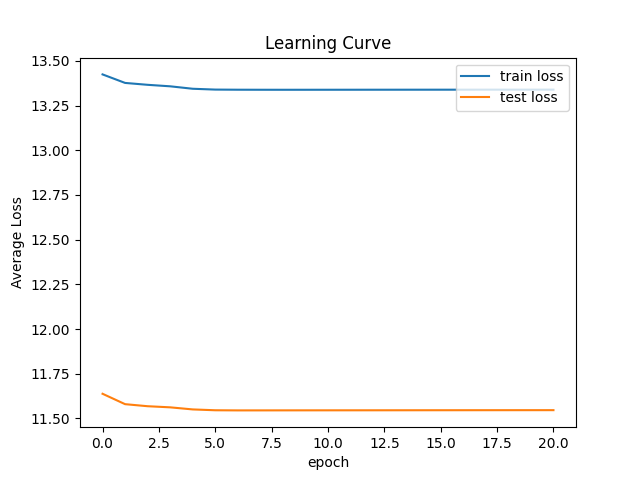
\includegraphics[width=0.6\textwidth]{../figs/learning_curve.png}
		\end{figure}

        \begin{center}
            \begin{tabular}{c | c}
                Epoch & Test Error \\ \hline
                1 & 89.9 \% \\
                2 & 90.88 \% \\
                3 & 91.68 \% \\
                4 & 92.45 \% \\
                5 & 92.89 \% \\
                6 & 93.25 \% \\
                7 & 93.3 \% \\
                8 & 93.62 \% \\
                9 & 93.66 \% \\
                10 & 93.64 \% \\
                11 & 93.58 \% \\
                12 & 93.57 \% \\
                13 & 93.62 \% \\
                14 & 93.65 \% \\
                15 & 93.67 \% \\
                16 & 93.58 \% \\
                17 & 93.58 \% \\
                18 & 93.61 \% \\
                19 & 93.62 \% \\
                20 & 93.59 \% \\
            \end{tabular}
        \end{center}

        Clearly there are some issues with my implementation.
        It seems like all the predictions tend to converge around equal probability for all outcomes.
        My hunch is that there is some step where I am inadvertently multiplying by index instead of matrix multiplication or vice versa but I was unable to figure out where.
    \end{soln}

    \item Implement the same network in PyTorch (or any other framework). You can use all the features of the framework e.g. auto-grad etc. Evaluate it on MNIST dataset, report test errors, and learning curve. (2 pts)
    
    \begin{soln}
        \begin{figure}[H]
			\centering
			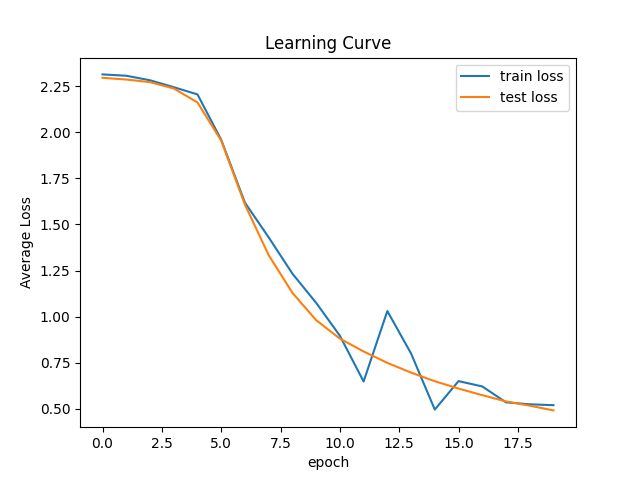
\includegraphics[width=0.6\textwidth]{../figs/pytorch_learning_curve.png}
		\end{figure}
       
        \begin{center}
            \begin{tabular}{c | c}
                Epoch & Test Error \\ \hline
                1 & 88.65 \% \\
                2 & 88.65 \% \\
                3 & 83.25 \% \\
                4 & 81.64 \% \\
                5 & 63.55 \% \\
                6 & 53.49 \% \\
                7 & 44.28 \% \\
                8 & 40.27 \% \\
                9 & 35.25 \% \\
                10 & 29.53 \% \\
                11 & 26.75 \% \\
                12 & 25.61 \% \\
                13 & 22.71 \% \\
                14 & 20.84 \% \\
                15 & 19.15 \% \\
                16 & 17.81 \% \\
                17 & 16.9 \% \\
                18 & 15.81 \% \\
                19 & 15.01 \% \\
                20 & 14.19 \% \\
            \end{tabular}
        \end{center}
    \end{soln}

    \item Try different weight initialization a) all weights initialized to 0, and b) initialize the weights randomly between -1 and 1. Report test error and learning curves for both. (You can use either of the implementations) (3 pts)
    
    \begin{soln}

        a) Initialized with zeros:

        \begin{figure}[H]
			\centering
			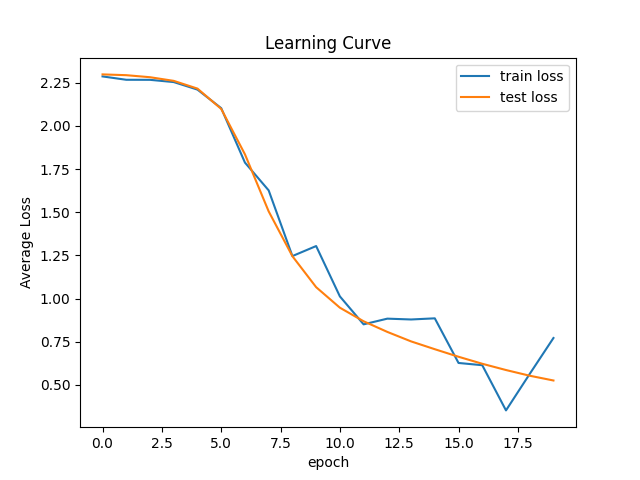
\includegraphics[width=0.6\textwidth]{../figs/init_zeros_learning_curve.png}
		\end{figure}
       
        \begin{center}
            \begin{tabular}{c | c}
                Epoch & Test Error \\ \hline
                1 & 88.65 \% \\
                2 & 87.76 \% \\
                3 & 72.9 \% \\
                4 & 63.61 \% \\
                5 & 75.4 \% \\
                6 & 59.54 \% \\
                7 & 56.38 \% \\
                8 & 47.47 \% \\
                9 & 40.43 \% \\
                10 & 35.47 \% \\
                11 & 30.63 \% \\
                12 & 27.47 \% \\
                13 & 24.58 \% \\
                14 & 23.43 \% \\
                15 & 21.48 \% \\
                16 & 19.67 \% \\
                17 & 18.34 \% \\
                18 & 16.75 \% \\
                19 & 16.01 \% \\
                20 & 15.17 \% \\
            \end{tabular}
        \end{center}

        b) Initialized with weights between -1 and 1:
        
        \begin{figure}[H]
			\centering
			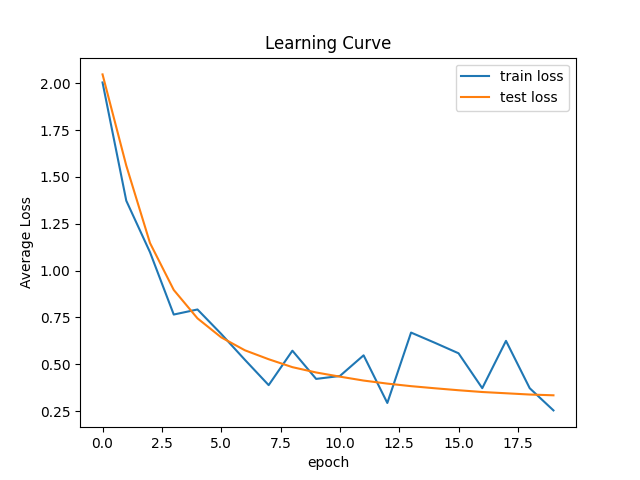
\includegraphics[width=0.6\textwidth]{../figs/neg_one_one_learning_curve.png}
		\end{figure}
       
        \begin{center}
            \begin{tabular}{c | c}
                Epoch & Test Error \\ \hline
                1 & 46.05 \% \\
                2 & 31.5 \% \\
                3 & 24.63 \% \\
                4 & 18.45 \% \\
                5 & 17.29 \% \\
                6 & 15.3 \% \\
                7 & 14.0 \% \\
                8 & 13.11 \% \\
                9 & 12.64 \% \\
                10 & 12.02 \% \\
                11 & 11.51 \% \\
                12 & 11.08 \% \\
                13 & 10.82 \% \\
                14 & 10.49 \% \\
                15 & 10.22 \% \\
                16 & 10.05 \% \\
                17 & 9.94 \% \\
                18 & 9.58 \% \\
                19 & 9.46 \% \\
                20 & 9.35 \% \\
            \end{tabular}
        \end{center}
    \end{soln}

\end{enumerate}

You should play with different hyperparameters like learning rate, batch size, etc. for your own learning. You only need to report results for any particular setting of hyperparameters. You should mention the values of those along with the results. Use $d_1 = 300$, $d_2 = 200$, $d_3 = 100$. For optimization use SGD (Stochastic gradient descent) without momentum, with some batch size say 32, 64, etc. MNIST can be obtained from here (https://pytorch.org/vision/ stable/datasets.html)

\bibliographystyle{apalike}
\end{document}
